\zchapter{UCC::Events}
UCC runs a lot of events. You should go to them! Dates and times may change. 
% Event with title and date
\newenvironment{event}[3]
{
	\begin{mdframed}[backgroundcolor=white]
	\color{black}{\section{#1}}
	\begin{mdframed}[backgroundcolor=white]
	When: #2
	\end{mdframed}
	\begin{mdframed}[backgroundcolor=white]
	Where: #3
	\end{mdframed}
	\begin{mdframed}[backgroundcolor=white]

	
}{\end{mdframed}\end{mdframed}}

% Simpler (no boxes)
%\renewenvironment{event}[3]
%{
%	\section{#1}
%	When: #2
	
%	Where: #3

%}{}




% By [XON]

\begin{event}{Fresher Welcome}{Friday, February 31st, 5:00PM}{Cameron Hall Loft (above the UCC clubroom)}
The Fresher welcome exists to welcome you, a new UCC member, to the club. There will be a number of current members there to talk with and get to know, and all of your questions about the club and how to use it will be answered. As a bonus, all first time members get {\bf FREE pizza}.
\end{event}

\begin{event}{Annual General Meeting}{Tuesday, March 11th, 1:00PM}{Guild Council Meeting Room}

The AGM is the meeting at which the new UCC committee is elected for 2014. The only way to be represented is to attend on the day. As a Fresher, you should attend to either run for or vote for the position of the Fresher Representative, who will be your liaison for the committee. If you don't know where the Guild Council Meeting Room is, arrive at the UCC clubroom a little early to join the mass exodus.

\end{event}

\begin{event}{Easter LAN}{Easter Weekend, 3:00PM until the morning after}{The Loft (above UCC Clubroom)}

UCC runs a number of LANs throughout the year, some with proper organisation, some without. The Easter LAN is the first big LAN of the academic year, taking place over the Easter weekend, the first weekend of mid-Semester one study break. We play a number of different games, and of course you can organise your own. LANs are free for all UCC members, but you can bring a friend for around \$5 (though of course you should encourage them to join). Bring your own PCs, or use one of the limited stock in the clubroom.

\end{event}


\begin{event}{LANs}{Throughout the Year, From Dusk til Dawn}{The Loft (above UCC Clubroom)}

The UCC hosts a number of more LANs throughout the year. As above, the Easter LAN is the first big one. Expect other LANs during the semester and breaks.

\end{event}

\begin{event}{Cameron Hall Quiz Night}{First Semester, probably in May, Evening}{UWA Tavern}

Bringing together the various clubs of Cameron Hall, the quiz night is the only proper time to use your smarts throughout your degree.

 (18+ Event).

\end{event}


\begin{event}{Camp}{18th to 21st July}{Lake Leshenaultia}

The UCC goes camping! Without tents. There is a dormitory. During the winter break, UCC will host a camp at Camp Leschenaultia. This is a chance to get your computer out of the house for a few days, tinkering and playing games with a whole bunch of other members. Don't worry, you won't be without precious internet.

 (18+ Event).

\end{event}
\pagebreak


\begin{event}{40th Anniversary Dinner}{Saturday, September 13th, 7.00 PM til late(r)}{South of Perth Yacht Club}

The big non-tech event of the year, the 40th Anniversary dinner is an opportunity for new members to meet the old blood of UCC, the ones that are still kicking on. Taking place in the lovely South of Perth Yacht Club, this fully catered dinner will be a good celebration of 40 years of computing. Expect entry prices to be around \$60 to \$80.

\end{event}

\begin{event}{Cameron Hall Charity Vigil}{Semester 2 - around mid-semester study break - From Dusk til Dawn}{Cameron Hall}

Once a year, all of the clubs in Cameron Hall get together and hold a night of fun and games to raise money for charity. While the details of the night are still to come, the UCC will probably host a LAN. There will be an entry fee for this event, but expect it to be fully worth it.

\end{event}


\begin{event}{Tech Talks}{Throughout the Year}{UCC Clubroom and/or the Loft}

Tech talks are a chance to demonstrate your own tech-y knowledge, or learn from someone else. Taking place throughout the year, as interest demands, the talks will cover a variety of topics, previous ones including introductions to TOR, learning basics, and the magic of data compression. Early on in the semester, a number of tech talks will cover learning to use the club's machines.

\end{event}

\pagebreak

\begin{mdframed}[backgroundcolor=white]
\color{black}{\section{FUCC Camp Scholarship}}
\color{black}{Incoming message from James Cox and Lionel Price:}


\color{black}{For new members to UCC, Lionel and I would like to tell you about our
full-ride scholarship program. We realise that Camp is fairly
expensive, but as once-freshers made good we are financially able to
provide unto others. Previous recipients of these scholarships have
gone onto great things so we are proud to offer it once more in 2014.
I would encourage everyone who is interested to take advantage of this
offer - I had a great time my first UCC Camp which is part of the
reason why I now offer this scholarship.

Two first-time UCC Campers will have their entry fee paid for by us.
As before, you will also obtain the privilege, if you should so wish,
to add a pink \textcolor{black}{F} to your UCC tags, denoting sophistication, intellect,
and exclusive membership of an elite group of teamkilling imbeciles.

To be eligible for this award, you must be a UWA student, member of
UCC, and to not have attended a previous UCC Camp. Applicants will
also need to declare in writing that they will participate in at least
one game of DotA during UCC Camp, and that when we play ET you will
not be a noob in the back with a mortar accomplishing nothing all
match.}
\end{mdframed}

\begin{figure}[H]
	\centering
	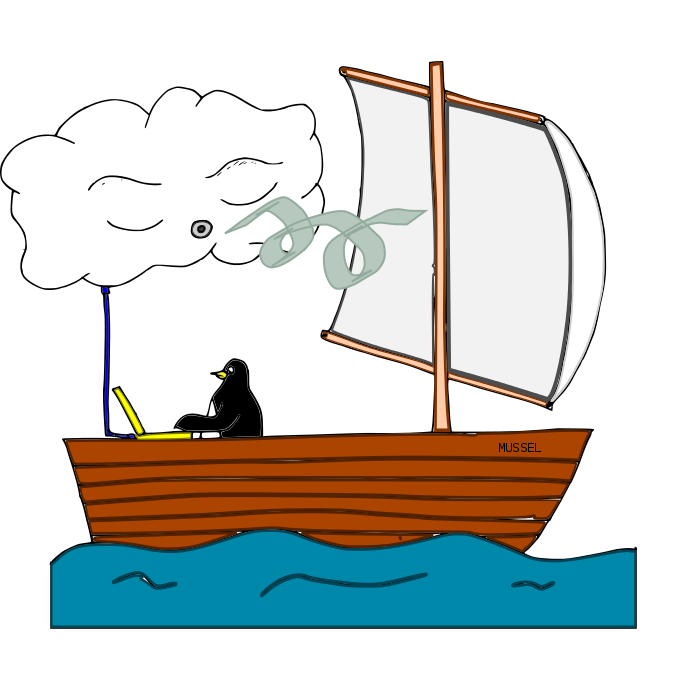
\includegraphics[width=0.8\textwidth]{figures/tux_boat.png}
	\caption{Tux enjoys Lake Leshenaultia at UCC::Camp \\ (Please note: There will not actually be watersports at the camp)}
	\label{tux_boat.png}
\end{figure}

